% Projektdokumentation – Gestensteuerung DENSO COBOTTA
% Übersetzen mit:  xelatex projektdokumentation.tex  (zweimal, für Verzeichnisse)
\documentclass[11pt,a4paper]{article}

\usepackage{fontspec}
\setmainfont{Latin Modern Roman}
\setsansfont{Latin Modern Sans}
\setmonofont{Latin Modern Mono}
\usepackage{polyglossia}
\setdefaultlanguage[spelling=new]{german}

\usepackage[a4paper,margin=2.5cm]{geometry}
\usepackage{graphicx}
\usepackage{booktabs}
\usepackage{tabularx}
\usepackage{array}
\usepackage{float}
\usepackage[font=small,labelfont=bf]{caption}
\usepackage{xcolor}
\usepackage{listings}
\usepackage{enumitem}
\usepackage{amsmath}
\usepackage{csquotes}
\usepackage[hidelinks]{hyperref}

\setlength{\parindent}{0pt}
\setlength{\parskip}{0.6em}
\setlist{itemsep=0.15em, topsep=0.3em}
% Für Deutsch sind in dieser TeX-Installation keine Trennmuster vorhanden,
% daher Flattersatz statt Blocksatz.
\emergencystretch=2em
\renewcommand{\arraystretch}{1.2}
\graphicspath{{abbildungen/}}

\newcommand{\datei}[1]{\texttt{#1}}

\lstset{basicstyle=\ttfamily\footnotesize, breaklines=true, frame=single, rulecolor=\color{gray},
        columns=fullflexible, keepspaces=true, showstringspaces=false,
        literate={–}{{\textendash}}1 {~}{{\textasciitilde}}1}

\begin{document}
\raggedright

% ---------------------------------------------------------------- Titelseite
\begin{titlepage}
\centering
\vspace*{4cm}
{\large Projektarbeit im Modul\\[0.3em] \textbf{Fabrikautomatisierung und Robotik}\par}
\vspace{1.5cm}
{\LARGE\bfseries Bildverarbeitungsgestützte Steuerung\\[0.3em] eines DENSO COBOTTA über Handgesten\par}
\vspace{2.5cm}
{\large
\begin{tabular}{rl}
Verfasser: & Abhinav Sridhar \\
\end{tabular}\par}
\vfill
\end{titlepage}

\tableofcontents
\newpage

% ---------------------------------------------------------------- 1
\section{Einleitung und Zielsetzung}

Industrieroboter werden üblicherweise über ein Handbediengerät (Teach Pendant) oder über
Programme gesteuert. Für das schnelle Positionieren oder für Demonstrationen ist eine
berührungslose Bedienung interessant: Der Bediener steuert den Roboter mit Handgesten vor einer
Kamera, ohne ein Gerät in der Hand zu halten.

Ziel dieser Projektarbeit ist ein System, das Handgesten über eine Webcam erkennt und in sichere
Bewegungsbefehle für einen DENSO COBOTTA umsetzt. Im Einzelnen:

\begin{itemize}
  \item Erkennung von Handgesten in Echtzeit mit der Bibliothek MediaPipe,
  \item Umsetzung der Gesten in Roboterbefehle nach dem Prinzip des Tippbetriebs am Teach Pendant,
  \item ein Sicherheitskonzept mit Freigabe, priorisiertem Stopp und Arbeitsraumgrenzen,
  \item Ansteuerung des realen COBOTTA über die Schnittstelle b-CAP aus Python,
  \item eine quantitative Auswertung der Gestenerkennung,
  \item ein eigener, auf selbst aufgenommenen Daten trainierter Gestenklassifikator im Vergleich
        zum vortrainierten MediaPipe-Modell sowie
  \item eine Dokumentation, mit der nachfolgende Studierende das System in Betrieb nehmen und
        weiterentwickeln können.
\end{itemize}

Die Software wurde so aufgebaut, dass sie ohne Roboter vollständig entwickelt und getestet werden
kann (simulierter Roboter) und für den realen Roboter nur das Roboter-Backend umgeschaltet wird.

% ---------------------------------------------------------------- 2
\section{Grundlagen}

\subsection{Handgestenerkennung mit MediaPipe}

MediaPipe ist eine quelloffene Bibliothek von Google für maschinelles Sehen. Der verwendete
\emph{Gesture Recognizer} arbeitet in drei Stufen: Zuerst wird eine Hand im Bild gefunden, dann
werden 21 Handpunkte (Landmarks, z.\,B. Fingerspitzen, Gelenke, Handgelenk) bestimmt, und
schließlich ordnet ein vortrainiertes Klassifikationsmodell die Handhaltung einer von sieben Gesten
zu: \emph{Open\_Palm}, \emph{Closed\_Fist}, \emph{Pointing\_Up}, \emph{Thumb\_Up},
\emph{Thumb\_Down}, \emph{Victory} und \emph{ILoveYou}. Erkennt das Modell keine dieser Gesten,
liefert es \emph{None}. Zu jeder Geste wird eine Konfidenz zwischen 0 und 1 ausgegeben.

Da das Modell bereits auf großen Datensätzen trainiert ist, ist für den Grundbetrieb kein eigenes
Training nötig. Die dritte Stufe lässt sich jedoch durch ein eigenes Modell ersetzen, das die
21 Handpunkte als Eingabe verwendet (Abschnitt~\ref{sec:klassifikator}). Die Erkennung läuft
lokal auf dem Rechner, ohne Internetverbindung.

\subsection{DENSO COBOTTA und b-CAP}

Der COBOTTA ist ein kompakter sechsachsiger Roboter von DENSO WAVE mit einer Reichweite von etwa
340\,mm. Er wird von einer RC8-Steuerung betrieben. Für die Ansteuerung von außen stellt DENSO das
Protokoll \emph{b-CAP} bereit, ein binäres Protokoll über TCP/IP (hier Port 5007). Über b-CAP
können Programme Verbindungen zur Steuerung aufbauen, die aktuelle Position lesen und
Bewegungsbefehle senden. DENSO stellt dafür einen quelloffenen Python-Client unter MIT-Lizenz
bereit\,\cite{orinbcap}, der in diesem Projekt verwendet wird.

\subsection{Tippbetrieb am Teach Pendant}

Beim manuellen Verfahren eines Industrieroboters (Tippbetrieb) wählt der Bediener am Teach Pendant
zunächst ein Koordinatensystem bzw. eine Achse und verfährt dann mit Plus- und Minus-Tasten in
kleinen Schritten oder kontinuierlich, bei reduzierter Geschwindigkeit. Die Schrittweite
(Inkrement) ist einstellbar. Dieses bekannte Bedienprinzip wurde auf die Gestensteuerung übertragen.

% ---------------------------------------------------------------- 3
\section{Systemkonzept}

\subsection{Anforderungen}

\begin{table}[H]
\centering
\begin{tabularx}{\textwidth}{>{\raggedright\arraybackslash}p{0.8cm}>{\raggedright\arraybackslash}X}
\toprule
Nr. & Anforderung \\
\midrule
A1 & Der Roboter lässt sich in X, Y und Z mit Handgesten verfahren. \\
A2 & Ein Stopp ist jederzeit mit einer einfachen Geste möglich und hat Vorrang vor allen anderen Befehlen. \\
A3 & Ohne bewusste Freigabe durch den Bediener bewegt sich der Roboter nicht. \\
A4 & Verlässt die Hand das Kamerabild, stoppt das System. \\
A5 & Der Roboter verlässt einen festgelegten Arbeitsraum nicht. \\
A6 & Unsichere oder kurzzeitige Erkennungen lösen keine Befehle aus. \\
A7 & Entwicklung und Test sind ohne Roboter möglich; für den realen Roboter wird nur das Roboter-Backend umgeschaltet. \\
A8 & Alle Parameter sind ohne Programmänderung in einer Konfigurationsdatei einstellbar. \\
\bottomrule
\end{tabularx}
\caption{Anforderungen an das System}
\end{table}

\subsection{Architektur}

Das System besteht aus einer Verarbeitungskette mit klar getrennten Komponenten
(Abbildung~\ref{fig:architektur}). Jede Komponente hat genau eine Aufgabe und eine eigene Datei.

\begin{figure}[H]
\centering
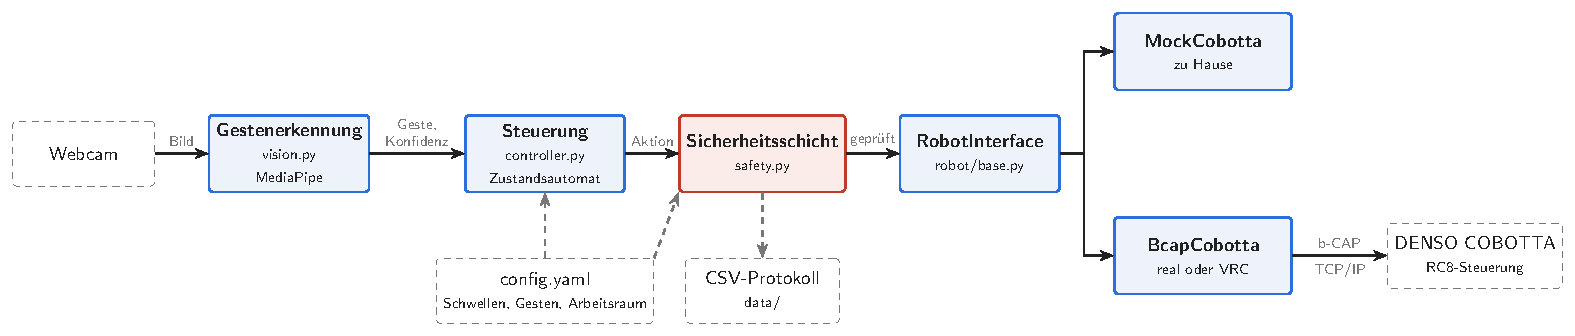
\includegraphics[width=\textwidth]{architektur.pdf}
\caption{Softwarearchitektur: Verarbeitungskette von der Kamera bis zum Roboter}
\label{fig:architektur}
\end{figure}

\begin{enumerate}
  \item \textbf{Gestenerkennung} (\datei{src/vision.py}): liest das Kamerabild und liefert je Bild die erkannte Geste und ihre Konfidenz.
  \item \textbf{Steuerung} (\datei{src/controller.py}): ein Zustandsautomat, der aus der Folge erkannter Gesten Aktionen erzeugt (Abschnitt~\ref{sec:zustandsautomat}).
  \item \textbf{Sicherheitsschicht} (\datei{src/safety.py}): prüft jede Aktion unabhängig von der Steuerung, bevor sie den Roboter erreicht.
  \item \textbf{Roboter-Schnittstelle} (\datei{src/robot/base.py}): eine abstrakte Klasse mit den Methoden \texttt{connect}, \texttt{get\_position}, \texttt{move\_relative}, \texttt{gripper}, \texttt{stop} und \texttt{disconnect}. Sie wird von einem simulierten Roboter (\texttt{MockCobotta}) und vom realen COBOTTA über b-CAP (\texttt{BcapCobotta}) implementiert.
\end{enumerate}

Durch die abstrakte Schnittstelle kann der Roboter ausgetauscht werden, ohne Gestenerkennung,
Steuerung oder Sicherheitslogik zu ändern. Welcher Roboter verwendet wird, legt allein der Eintrag
\texttt{roboter.backend} in \datei{config.yaml} fest.

\subsection{Gestenkonzept}

\begin{table}[H]
\centering
\begin{tabularx}{\textwidth}{>{\raggedright\arraybackslash}p{3.6cm}>{\raggedright\arraybackslash}p{3.2cm}>{\raggedright\arraybackslash}X}
\toprule
Geste & MediaPipe-Name & Befehl \\
\midrule
Offene Hand & Open\_Palm & STOPP (höchste Priorität) \\
Faust (halten) & Closed\_Fist & Freigabe nach Start und nach jedem Stopp; sonst keine Aktion \\
Zeigefinger oben & Pointing\_Up & aktive Achse wechseln X $\rightarrow$ Y $\rightarrow$ Z \\
Daumen hoch & Thumb\_Up & ein Schritt in positiver Richtung der aktiven Achse \\
Daumen runter & Thumb\_Down & ein Schritt in negativer Richtung der aktiven Achse \\
I-love-you-Zeichen & ILoveYou & Schrittweite umschalten 5\,mm $\leftrightarrow$ 1\,mm \\
Victory-Zeichen & Victory & Greifer öffnen/schließen \\
\bottomrule
\end{tabularx}
\caption{Zuordnung der Gesten zu Befehlen}
\label{tab:gesten}
\end{table}

Begründung der Gestaltung:
\begin{itemize}
  \item \textbf{Achse wählen, dann verfahren:} entspricht dem Tippbetrieb am Teach Pendant und ist
        damit für Anwender aus der Robotik vertraut.
  \item \textbf{Nur vortrainierte Gesten:} Die sieben MediaPipe-Gesten sind auf großen Datensätzen
        trainiert und daher robust. Eine Steuerung mit je einer Geste pro Achsrichtung würde neun
        Gesten erfordern und damit ein eigenes Modell sowie mehr Verwechslungsmöglichkeiten.
  \item \textbf{Diskrete Schritte statt Handposition:} Eine Steuerung über die Position der Hand im
        Bild wäre intuitiver, aber ungenau (Tiefe nur schwer bestimmbar) und würde jede unbeabsichtigte
        Handbewegung an den Roboter weitergeben. Feste Schritte sind vorhersehbar.
  \item \textbf{Offene Hand als Stopp:} allgemein verständliches Haltezeichen.
  \item \textbf{Faust halten als Freigabe:} eine bewusste Handlung, die nicht versehentlich entsteht.
  \item \textbf{Achsfarben:} Die aktive Achse wird in der in Robotik und CAD üblichen Farbkonvention
        angezeigt: X rot, Y grün, Z blau.
  \item \textbf{Grob- und Feinschritt:} 5\,mm zum zügigen Annähern, 1\,mm zum genauen Positionieren,
        entsprechend dem einstellbaren Inkrement am Teach Pendant.
\end{itemize}

\subsection{Zustandsautomat}
\label{sec:zustandsautomat}

Die Steuerung kennt zwei Zustände (Abbildung~\ref{fig:zustand}). Nach dem Start befindet sie sich
im Zustand GESTOPPT; Bewegungen sind erst nach einer Freigabe möglich.

\begin{figure}[H]
\centering
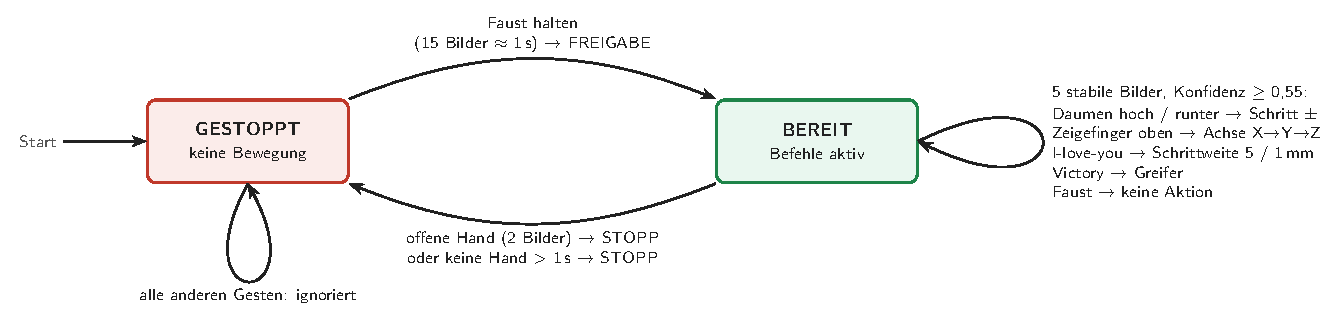
\includegraphics[width=\textwidth]{zustandsautomat.pdf}
\caption{Zustandsautomat der Steuerung}
\label{fig:zustand}
\end{figure}

Damit Erkennungsfehler einzelner Bilder keine Befehle auslösen, wird ein Befehl erst ausgeführt,
wenn dieselbe Geste in mehreren aufeinanderfolgenden Bildern mit ausreichender Konfidenz erkannt
wurde (Entprellung). Zwei Arten von Befehlen werden unterschieden:
\begin{itemize}
  \item \textbf{Tippbetrieb:} Schritt plus/minus wiederholt sich beim Halten der Geste im Takt der
        Sperrzeit (0,5\,s). Eine kurz gezeigte Geste erzeugt genau einen Schritt.
  \item \textbf{Flankengesteuert:} Achswechsel, Schrittweite und Greifer werden je gezeigter Geste
        nur einmal ausgeführt, auch wenn die Geste länger gehalten wird. So springt die Achse beim
        Halten nicht unkontrolliert weiter.
\end{itemize}

\subsection{Sicherheitskonzept}
\label{sec:sicherheit}

\begin{table}[H]
\centering
\begin{tabularx}{\textwidth}{>{\raggedright\arraybackslash}p{4.3cm}>{\raggedright\arraybackslash}X}
\toprule
Maßnahme & Umsetzung und Begründung \\
\midrule
Start im Zustand GESTOPPT & Nach dem Programmstart ist keine Bewegung möglich (A3). \\
Freigabe durch Faust & Faust ca. 1\,s halten (15 Bilder). Bewusste Handlung, entsteht nicht zufällig. \\
Priorisierter Stopp & Offene Hand stoppt nach 2 Bildern, in jedem Zustand und vor allen anderen Befehlen (A2). \\
Niedrigere Schwelle für Stopp (fail-safe) & Stopp ab Konfidenz 0,45, alle anderen Befehle erst ab 0,55. Ein unnötiger Stopp ist harmlos, ein verpasster Stopp gefährlich. \\
Quittierung & Nach jedem Stopp ist eine erneute Freigabe nötig. \\
Überwachung der Hand & Ist länger als 1\,s keine Hand sichtbar, stoppt das System (A4). \\
Entprellung & Befehle erst nach 5 aufeinanderfolgenden Bildern mit Konfidenz $\geq$ 0,55 (A6). \\
Sicherheitsschicht (Redundanz) & Prüft unabhängig von der Steuerung: Freigabe vorhanden, Schritt $\leq$ 10\,mm, Zielposition im Arbeitsraum (A5). Unzulässige Befehle werden abgelehnt und protokolliert. \\
Reduzierte Geschwindigkeit & Der reale Roboter fährt mit 10\,\% der Geschwindigkeit. \\
Hardware-Not-Halt & Bleibt jederzeit wirksam und ist der Software übergeordnet. \\
\bottomrule
\end{tabularx}
\caption{Maßnahmen des Sicherheitskonzepts}
\end{table}

Das Sicherheitskonzept ist mehrstufig: Steuerung und Sicherheitsschicht prüfen unabhängig
voneinander, und die Sicherheitsfunktionen des Roboters selbst (Not-Halt, Kraftbegrenzung des
kollaborierenden Roboters) bleiben unberührt. Es handelt sich um eine Software-Absicherung für den
Versuchs- und Demonstrationsbetrieb, nicht um eine zertifizierte Sicherheitsfunktion im Sinne der
Maschinensicherheit.

% ---------------------------------------------------------------- 4
\section{Umsetzung}

\subsection{Entwicklungsumgebung und Softwarestruktur}

Die Software ist in Python 3.11 geschrieben und wurde auf einem MacBook Air (Apple M3) mit der
eingebauten Webcam entwickelt. Verwendete Bibliotheken: MediaPipe (Gestenerkennung), OpenCV
(Kamera und Anzeige), PyYAML (Konfiguration), Matplotlib (Diagramme), scikit-learn (eigener
Klassifikator) sowie der b-CAP-Client von DENSO WAVE.

\begin{table}[H]
\centering
\small
\begin{tabularx}{\textwidth}{>{\raggedright\arraybackslash}p{6.1cm}>{\raggedright\arraybackslash}X}
\toprule
Datei & Aufgabe \\
\midrule
\datei{main.py} & Hauptprogramm: verbindet alle Komponenten, Anzeige, Protokoll \\
\datei{gesture\_demo.py} & nur Gestenerkennung, ohne Roboter \\
\datei{config.yaml} & alle Einstellungen \\
\datei{src/vision.py} & Kamera und MediaPipe-Gestenerkennung \\
\datei{src/klassifikator.py} & Merkmale und eigener Gestenklassifikator \\
\datei{src/controller.py} & Zustandsautomat: Geste $\rightarrow$ Aktion \\
\datei{src/safety.py} & Sicherheitsschicht \\
\datei{src/robot/base.py} & abstrakte Roboter-Schnittstelle \\
\datei{src/robot/mock.py} & simulierter COBOTTA \\
\datei{src/robot/bcap\_cobotta.py} & realer COBOTTA über b-CAP \\
\datei{third\_party/bCAPClient/} & b-CAP-Client von DENSO WAVE (MIT-Lizenz) \\
\datei{scripts/test\_steuerung.py} & automatischer Test von Steuerung und Sicherheitsschicht \\
\datei{scripts/test\_bcap\_verbindung.py} & schrittweiser Verbindungstest (Simulation oder realer Roboter) \\
\datei{scripts/aufnahme\_erkennung.py} & geführte Aufnahme für die Auswertung \\
\datei{scripts/analyse\_erkennung.py} & Auswertung der Gestenerkennung \\
\datei{scripts/analyse\_protokoll.py} & Auswertung der Protokolle von \datei{main.py} \\
\datei{scripts/aufnahme\_datensatz.py} & Datensatz für den eigenen Klassifikator aufnehmen \\
\datei{scripts/training\_klassifikator.py} & Training, Validierung, Vergleich mit MediaPipe \\
\datei{scripts/vergleich\_merkmale.py} & Vergleich Rohkoordinaten / Formmerkmale \\
\datei{scripts/test\_klassifikator.py} & automatischer Test der Merkmalsberechnung \\
\bottomrule
\end{tabularx}
\caption{Dateien des Projekts}
\end{table}

\subsection{Gestenerkennung}

Der MediaPipe Gesture Recognizer wird im Video-Modus mit einer Hand betrieben. Jedes Kamerabild
wird gespiegelt (natürlicheres Gestikulieren, wie vor einem Spiegel) und mit einem streng
steigenden Zeitstempel an das Modell übergeben. Da die Kamera unter macOS beim Start oft einige
leere Bilder liefert, wartet die Kamera-Klasse bis zu 2\,s auf gültige Bilder und gibt sonst eine
Fehlermeldung mit möglichen Ursachen aus.

Über \texttt{erkennung.backend} in \datei{config.yaml} wird festgelegt, wer die Geste zuordnet:
der vortrainierte MediaPipe-Klassifikator (\texttt{mediapipe}, Standard) oder das eigene Modell
(\texttt{eigen}, Abschnitt~\ref{sec:klassifikator}). Beide liefern dieselben Gestennamen und eine
Konfidenz, sodass Steuerung und Sicherheitsschicht unverändert bleiben.

\subsection{Steuerung}

Die Klasse \texttt{GestureController} erhält je Bild die erkannte Geste, die Konfidenz und die Zeit
und gibt eine Liste von Aktionen zurück (\texttt{FREIGABE}, \texttt{STOPP}, \texttt{BEWEGEN},
\texttt{ACHSE}, \texttt{SCHRITTWEITE}, \texttt{GREIFER}). Sie zählt, in wie vielen
aufeinanderfolgenden Bildern dieselbe Geste über der Schwelle erkannt wurde, und vergleicht diesen
Zähler mit den Grenzwerten aus der Konfiguration. Die Steuerung kennt keinen Roboter; sie erzeugt
nur Aktionen. Dadurch lässt sie sich ohne Kamera und Roboter automatisch testen.

\subsection{Sicherheitsschicht}

Die Klasse \texttt{SafetyLayer} führt Aktionen nur aus, wenn sie zulässig sind. Für eine
Bewegung liest sie die aktuelle Position vom Roboter, berechnet die Zielposition und prüft sie gegen
die Arbeitsraumgrenzen. Jede Aktion liefert ein Ergebnis (ausgeführt/abgelehnt) und eine Meldung,
die angezeigt und protokolliert wird.

\subsection{Anbindung des COBOTTA über b-CAP}

Die Klasse \texttt{BcapCobotta} verwendet den Python-Client von DENSO WAVE. Ablauf:
\begin{enumerate}
  \item TCP-Verbindung zur RC8-Steuerung (IP-Adresse 192.168.0.1, Port 5007, laut Lehrveranstaltungsprojekt),
  \item Controller-Verbindung (Provider \texttt{CaoProv.DENSO.VRC} wie im Python-Beispiel von DENSO,
        einstellbar in \datei{config.yaml}) und Roboter-Objekt \texttt{Arm},
  \item Fehler quittieren, Armberechtigung holen (\texttt{TakeArm}), Motor einschalten,
  \item reduzierte Geschwindigkeit setzen (\texttt{ExtSpeed}, 10\,\%),
  \item Position über die Variable \texttt{@CURRENT\_POSITION} lesen,
  \item Schritte als Linearbewegung zu einer Zielpose
        \texttt{P(X, Y, Z, Rx, Ry, Rz, Fig)} = aktuelle Pose + Schritt, mit unveränderter Orientierung,
  \item Stopp über \texttt{Halt}; beim Beenden Motor aus und Armberechtigung abgeben.
\end{enumerate}
Bewegt wird mit der DENSO-Bewegungsoption \texttt{@E} (einstellbar über \texttt{bewegung.bahnende}):
Der Aufruf kehrt erst zurück, wenn der Roboter das Ziel erreicht hat. Die Schritte werden also
synchron ausgeführt. In der Simulation dauert ein 5-mm-Schritt bei 10\,\% Geschwindigkeit 0,58\,s,
ein 1-mm-Schritt 0,26\,s (Abschnitt~\ref{sec:simulation}).

\textbf{Erfahrungen aus der Inbetriebnahme in der Simulation.} Die Anbindung wurde mit der
virtuellen Robotersteuerung VRC von DENSO erprobt
(Abschnitt~\ref{sec:simulation}). Dabei ergaben sich zwei Korrekturen am Code:
\begin{itemize}
  \item \textbf{Provider:} Zunächst war \texttt{CaoProv.DENSO.RC8} eingetragen. Das Python-Beispiel
        von DENSO für eine direkte b-CAP-Verbindung verwendet jedoch \texttt{CaoProv.DENSO.VRC};
        damit gelang die Verbindung auf Anhieb. Der Wert steht jetzt in \datei{config.yaml}.
  \item \textbf{Bewegungsoption:} Mit der zunächst verwendeten Option \texttt{@P} (Überschleifen)
        meldete die Steuerung den Schritt bereits als beendet, als der Roboter erst 2,9 der 5\,mm
        zurückgelegt hatte. Mit \texttt{@E} wurden 4,998\,mm gemessen, nach dem Rückweg betrug die
        Abweichung zur Startposition 0,000\,mm.
\end{itemize}

\subsection{Konfiguration und Protokollierung}

Alle Einstellungen stehen in \datei{config.yaml} (Anhang~\ref{anh:config}): Kamera,
Konfidenzschwellen, Entprellung, Zuordnung der Gesten, Schrittweiten, Geschwindigkeit,
Arbeitsraum, Roboterverbindung und Greifer. Jeder Lauf von \datei{main.py} wird in
\datei{data/protokoll\_<datum\_uhrzeit>.csv} protokolliert: Zeit, Geste, Konfidenz, Zustand, Aktion,
Ergebnis, Meldung, Reaktionszeit, Ausführungsdauer und Position.

% ---------------------------------------------------------------- 5
\section{Test und Auswertung}

\subsection{Automatisierte Tests der Steuerung}

Das Skript \datei{scripts/test\_steuerung.py} spielt simulierte Gestenfolgen mit 30 Bildern pro
Sekunde durch Steuerung und Sicherheitsschicht und prüft das Verhalten gegen das
Sicherheitskonzept. Alle 21 Prüfungen sind bestanden, unter anderem:
\begin{itemize}
  \item Start im Zustand GESTOPPT; ohne Freigabe keine Bewegung,
  \item kurze Faust (0,2\,s) gibt nicht frei; gehaltene Faust gibt frei,
  \item zu kurze Gesten (0,1\,s) und Bewegungsgesten mit Konfidenz 0,5 lösen nichts aus,
  \item Achswechsel, Schrittweite und Greifer schalten nur einmal pro Geste,
  \item Stopp nach 0,1\,s, auch bei Konfidenz 0,5; danach keine Bewegung ohne neue Freigabe,
  \item kein Stopp bei 0,8\,s ohne Hand, automatischer Stopp nach mehr als 1\,s,
  \item die Arbeitsraumgrenze wird nicht überschritten; Schritte darüber hinaus werden abgelehnt.
\end{itemize}

\subsection{Versuchsaufbau zur Gestenerkennung}

Mit \datei{scripts/aufnahme\_erkennung.py} wurde jede der sieben Gesten jeweils 2\,s lang
aufgenommen und jedes Bild protokolliert (erkannte Geste, Konfidenz, Rechenzeit). Die Aufnahmen
erfolgten mit der eingebauten Webcam eines MacBook Air (M3) unter vier Bedingungen: helles bzw.
gedimmtes Licht, jeweils mit 50\,cm und 100\,cm Abstand der Hand zur Kamera. Die Bedingung
\enquote{hell, 50\,cm} wurde wiederholt (siehe unten). Die Videoeffekte von macOS (Reaktionen,
Center Stage, Porträt) waren ausgeschaltet, da sie direkt ins Kamerabild gezeichnet werden.
Die Gesten-Aufnahmen umfassen insgesamt 1416 Bilder. Zusätzlich wurden 60\,s freie Handbewegung
ohne beabsichtigte Befehlsgesten aufgenommen (1027 Bilder).

Als \enquote{richtig erkannt} gilt ein Bild, wenn MediaPipe die gezeigte Geste mit einer Konfidenz
über der jeweiligen Schwelle erkennt (0,55 bzw. 0,45 für den Stopp).

\subsection{Erkennungsrate}

\begin{table}[H]
\centering
\begin{tabular}{lrrr}
\toprule
Geste & Bilder & Erkennungsrate & mittlere Konfidenz \\
\midrule
Offene Hand & 181 & 100,0\,\% & 0,62 \\
Zeigefinger oben & 180 & 96,7\,\% & 0,80 \\
Daumen hoch & 211 & 100,0\,\% & 0,67 \\
Daumen runter & 211 & 100,0\,\% & 0,91 \\
Victory & 212 & 100,0\,\% & 0,86 \\
Faust & 210 & 82,4\,\% & 0,81 \\
I love you & 211 & 100,0\,\% & 0,76 \\
\midrule
\textbf{gesamt} & 1416 & \textbf{97,0\,\%} & \\
\bottomrule
\end{tabular}
\caption{Erkennungsrate je Geste über alle Bedingungen (mittlere Konfidenz der richtig erkannten Bilder)}
\end{table}

\begin{table}[H]
\centering
\small
\begin{tabular}{lrrrrr}
\toprule
Geste & dunkel 100\,cm & dunkel 50\,cm & hell 100\,cm & hell 50\,cm & hell 50\,cm (Wdh.) \\
\midrule
Offene Hand & 100,0\,\% & 100,0\,\% & 100,0\,\% & 100,0\,\% & 100,0\,\% \\
Zeigefinger oben & 100,0\,\% & 100,0\,\% & 83,9\,\% & 100,0\,\% & 98,3\,\% \\
Daumen hoch & 100,0\,\% & 100,0\,\% & 100,0\,\% & 100,0\,\% & 100,0\,\% \\
Daumen runter & 100,0\,\% & 100,0\,\% & 100,0\,\% & 100,0\,\% & 100,0\,\% \\
Victory & 100,0\,\% & 100,0\,\% & 100,0\,\% & 100,0\,\% & 100,0\,\% \\
Faust & 100,0\,\% & 100,0\,\% & 100,0\,\% & 38,3\,\% & 100,0\,\% \\
I love you & 100,0\,\% & 100,0\,\% & 100,0\,\% & 100,0\,\% & 100,0\,\% \\
\bottomrule
\end{tabular}
\caption{Erkennungsrate je Geste und Aufnahmebedingung}
\label{tab:bedingungen}
\end{table}

Fünf der sieben Gesten wurden unter allen Bedingungen in jedem Bild erkannt. Die Faust erreichte
in der ersten Aufnahme \enquote{hell, 50\,cm} nur 38,3\,\%; in den übrigen Fällen wurde sie
nicht als andere Geste, sondern als \enquote{keine Geste} eingestuft. Die Wiederholung unter
gleichen Bedingungen ergab 100\,\% bei einer mittleren Konfidenz von 0,90. Die Ursache lag daher
wahrscheinlich in der Handhaltung der ersten Aufnahme (zu nah an der Kamera oder schräg gehalten),
nicht im System. Beide Aufnahmen gehen in die Gesamtwerte ein.

\begin{figure}[H]
\centering
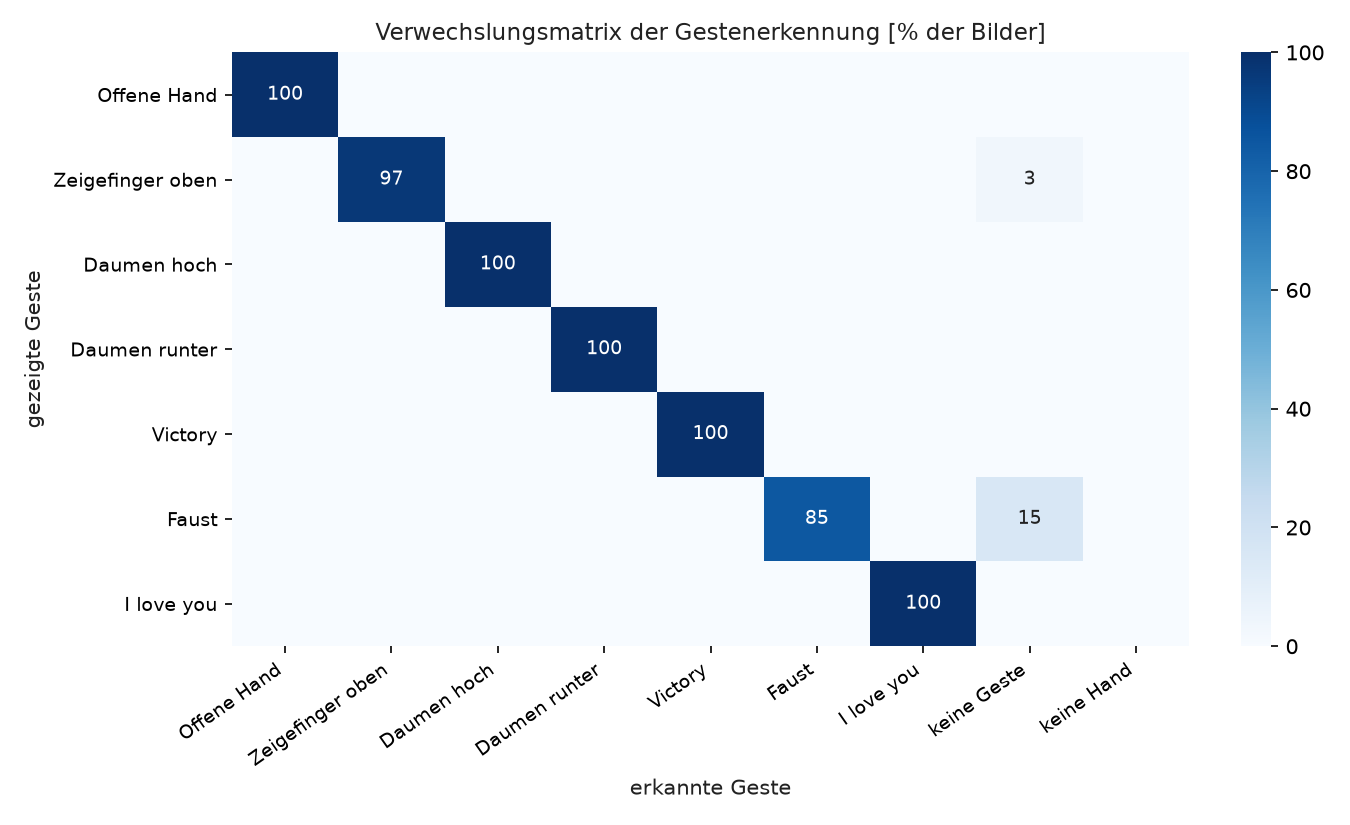
\includegraphics[width=0.92\textwidth]{verwechslungsmatrix.png}
\caption{Verwechslungsmatrix: Anteil der Bilder je gezeigter (Zeile) und erkannter Geste (Spalte)}
\label{fig:matrix}
\end{figure}

Die Verwechslungsmatrix (Abbildung~\ref{fig:matrix}) zeigt das wichtigste Ergebnis für die
Sicherheit: \textbf{Keine Geste wurde als eine andere Geste erkannt.} Alle 43 nicht richtig
erkannten Bilder waren \enquote{keine Geste}, \enquote{keine Hand} oder die richtige Geste knapp
unter der Schwelle. Ein Erkennungsfehler führt damit zu \emph{keiner} Aktion, nicht zu einer
falschen.

\subsection{Auslösung auf Befehlsebene}

Jede Aufnahme wurde zusätzlich durch den Zustandsautomaten gespielt. Ausgewertet wurde, ob der
richtige Befehl ausgelöst wird und nach welcher Zeit. Die Zeit zählt ab dem ersten aufgenommenen
Bild, in dem die Geste bereits gezeigt wird, und entspricht damit der Entprellzeit der Steuerung.

\begin{table}[H]
\centering
\begin{tabular}{lrrr}
\toprule
Geste & richtiger Befehl & mittlere Auslösezeit & falsche Befehle \\
\midrule
Offene Hand (Stopp) & 5 / 5 & 60\,ms & 0 \\
Zeigefinger oben & 5 / 5 & 239\,ms & 0 \\
Daumen hoch & 5 / 5 & 213\,ms & 0 \\
Daumen runter & 5 / 5 & 213\,ms & 0 \\
Victory & 5 / 5 & 214\,ms & 0 \\
Faust (Freigabe) & 4 / 5 & 816\,ms & 0 \\
I love you & 5 / 5 & 214\,ms & 0 \\
\bottomrule
\end{tabular}
\caption{Auslösung der Befehle bei Simulation der Aufnahmen durch die Steuerung}
\end{table}

In 34 von 35 Aufnahmen wurde der richtige Befehl ausgelöst, falsche Befehle traten nicht auf. Die
fehlende Freigabe betrifft die oben beschriebene erste Faust-Aufnahme. Der Stopp reagiert wie
beabsichtigt deutlich schneller als alle anderen Befehle.

\subsection{Rechenzeit und Bildrate}

Die Gestenerkennung benötigt im Mittel 12,9\,ms pro Bild (Median 14,1\,ms, 95-\%-Quantil
14,9\,ms, Maximum 27,9\,ms). Die Kamera liefert dagegen nur 15 Bilder pro Sekunde (Median; bis
30 Bilder pro Sekunde bei hellem Licht), da die Belichtungsautomatik bei wenig Licht die Bildrate
senkt. Die Reaktionszeit wird also durch die Kamera begrenzt, nicht durch die Erkennung. Bei
15 Bildern pro Sekunde ergeben sich Entprellzeiten von etwa 270\,ms für Bewegungsbefehle,
70\,ms für den Stopp und 0,9\,s für die Freigabe.

\subsection{Fehlauslösungen bei freier Handbewegung}

Während 60\,s natürlicher Handbewegung (Gestikulieren, Gesicht berühren, Tippen) wurde im
ungünstigsten Fall, also bei durchgehend freigegebenem System, \textbf{kein einziger Bewegungsbefehl}
und kein sonstiger Befehl ausgelöst. Es traten 16 Stopps auf, da eine offene Hand beim
Gestikulieren häufig vorkommt. Diese Stopps sind harmlos und die bewusste Folge der niedrigen
Stopp-Schwelle (fail-safe): Das System stoppt lieber einmal zu oft als einmal zu wenig.

\subsection{Erprobung in der Simulation}
\label{sec:simulation}

Die vollständige Kette -- Kamera, Erkennung, Steuerung, Sicherheitsschicht und
b-CAP-Anbindung -- wurde mit der virtuellen Robotersteuerung VRC von DENSO erprobt. Die Simulation läuft in einer Windows-11-VM (UTM) auf dem MacBook, mit dem
Beispielprojekt \datei{Cobotta\_test.WPJ} (COBOTTA CVR038A1). Als b-CAP-Server dient der
\emph{bCapListener} aus ORiN2. \datei{main.py} läuft unverändert auf dem Mac mit der Webcam und
verbindet sich über das virtuelle Netzwerk mit der VM (Abbildung~\ref{fig:vrc}). Gegenüber dem
realen Roboter ändern sich nur die IP-Adresse und das Roboter-Backend
(\texttt{--roboter bcap --ip <IP der VM>}).

\begin{figure}[H]
\centering
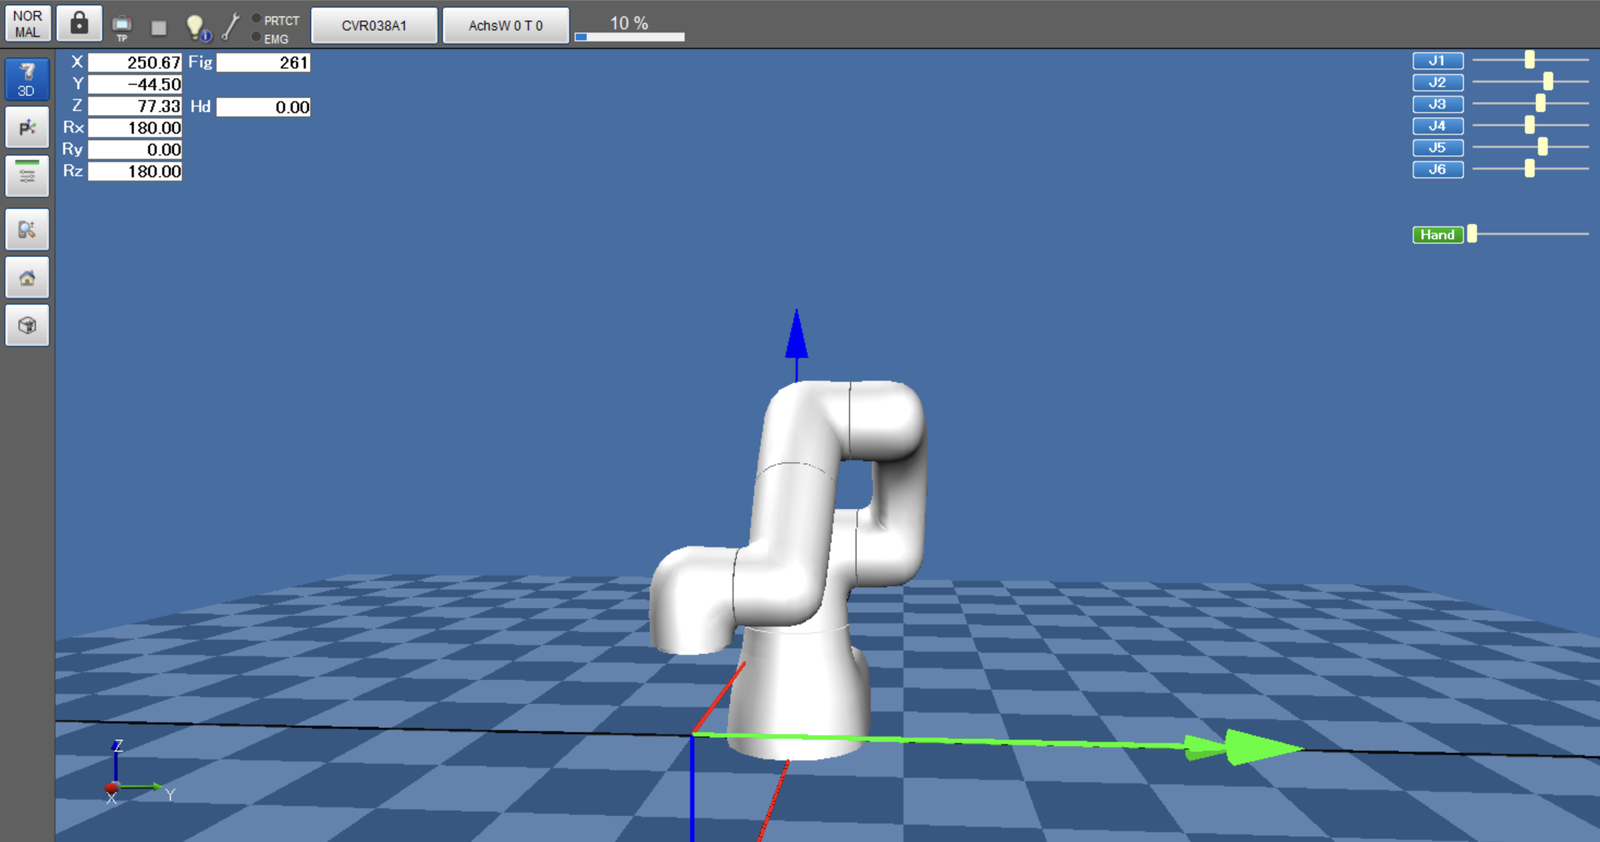
\includegraphics[width=0.85\textwidth]{simulation_vrc.png}
\caption{Simulierter COBOTTA in der virtuellen Steuerung VRC (virtuelles Teach Pendant mit 3D-Ansicht)}
\label{fig:vrc}
\end{figure}

\textbf{Verbindungstest} (\datei{scripts/test\_bcap\_verbindung.py}): Verbindung, Lesen der
Position und Halt funktionierten. Ein Schritt von 5\,mm in Z ergab 4,998\,mm in 0,59\,s; nach dem
Rückweg lag die Abweichung zur Startposition bei 0,000\,mm.

\textbf{Gestensteuerung:} In zwei Läufen von zusammen 7,3\,min wurden 322 Aktionen ausgeführt und
mit \datei{scripts/analyse\_protokoll.py} ausgewertet (\datei{docs/auswertung/ergebnis\_simulation.md}).

\begin{table}[H]
\centering
\small
\begin{tabular}{lrrr}
\toprule
Aktion & Anzahl (ausgeführt) & Auslösezeit (Median) & Ausführung (Median) \\
\midrule
Freigabe (Faust) & 14 (14) & 468\,ms & -- \\
Stopp (offene Hand) & 11 (11) & 35\,ms & 0,7\,ms \\
Stopp (keine Hand sichtbar) & 7 (7) & 978\,ms & 0,8\,ms \\
Schritt 5\,mm / 1\,mm & 269 (236) & 167\,ms & 583\,ms / 263\,ms \\
Achse wechseln & 11 (11) & 265\,ms & -- \\
Schrittweite umschalten & 8 (8) & 268\,ms & -- \\
\bottomrule
\end{tabular}
\caption{Gestensteuerung des simulierten COBOTTA (10\,\% Geschwindigkeit). Auslösezeit: erstes Bild
der Geste bis zum Befehl; beim Stopp ohne Hand planmäßig nach der Wartezeit von 1\,s.}
\label{tab:simulation}
\end{table}

Ergebnisse:
\begin{itemize}
  \item \textbf{Schrittgenauigkeit:} Alle 236 ausgeführten Schritte entsprachen der Soll-Schrittweite
        (Abweichung 0,0\,mm bei 0,1\,mm Auflösung des Protokolls). Abgedeckt waren alle drei Achsen in
        beiden Richtungen mit beiden Schrittweiten (12 Kombinationen).
  \item \textbf{Arbeitsraum:} 33 Schritte wurden von der Sicherheitsschicht abgelehnt, weil sie die
        Grenzen X\,=\,300, Y\,=\,150 bzw. Z\,=\,250\,mm überschritten hätten. Der Roboter blieb an der
        Grenze stehen.
  \item \textbf{Keine Fehlbefehle:} Bei bewusst ungeordneter Handbewegung zwischen den Gesten
        (5 Versuche) wurde kein Befehl ausgelöst.
  \item \textbf{Stopp während eines Schritts:} Da die Schritte synchron ausgeführt werden, wertet das
        Programm während eines Schritts keine Kamerabilder aus. Ein Stopp wirkt daher erst nach dem
        laufenden Schritt: im ungünstigsten Fall nach der Restdauer des Schritts (bis 0,58\,s bei
        5\,mm, bis 0,26\,s bei 1\,mm) plus etwa 35\,ms. Nach dem letzten Schritt bewegte sich der
        Roboter in allen Versuchen nicht weiter, auch wenn die offene Hand erst einige Sekunden später
        erkannt wurde.
\end{itemize}

Nicht abgedeckt: der Greifer (in \datei{config.yaml} deaktiviert, es wurde nur die Logik geprüft),
die unteren Arbeitsraumgrenzen sowie die Ende-zu-Ende-Latenz bis zur tatsächlichen Bewegung, die
nur am realen Roboter mit einer Zeitlupenaufnahme messbar ist. Die Arbeitsraumgrenzen sind
Beispielwerte und müssen vor einem Einsatz am realen Roboter an den Aufbau angepasst werden.

% ---------------------------------------------------------------- 6
\section{Eigener Gestenklassifikator}
\label{sec:klassifikator}

\subsection{Ziel und Vorgehen}

Zusätzlich zum vortrainierten MediaPipe-Klassifikator wurde ein eigenes Modell entwickelt.
MediaPipe liefert weiterhin die Hand und ihre 21 Punkte; nur die Zuordnung zu einer Geste
übernimmt das eigene Modell. Ziel war, den vollständigen Ablauf des überwachten Lernens selbst
umzusetzen (Datenerhebung, Merkmale, Vergleich mehrerer Verfahren, Validierung, unabhängiger
Test) und das Ergebnis messbar mit MediaPipe zu vergleichen.

Das Modell unterscheidet acht Klassen: die sieben Befehlsgesten und \enquote{keine
Befehlsgeste}. Die achte Klasse ist notwendig, da ein Klassifikator sonst jede Handhaltung,
z.\,B. eine locker gehaltene Hand, der ähnlichsten Befehlsgeste zuordnen würde. Sie wird wie
\emph{None} bei MediaPipe behandelt und löst keine Aktion aus. Als Konfidenz dient die
Klassenwahrscheinlichkeit des Modells; es gelten dieselben Schwellen wie für MediaPipe.

\subsection{Datensatz}

Mit \datei{scripts/aufnahme\_datensatz.py} wurde jede Klasse 10\,s lang aufgenommen. Gespeichert
werden nur die 21 Handpunkte (MediaPipe-Weltkoordinaten in Metern), keine Bilder, sowie zum
Vergleich das Ergebnis des MediaPipe-Klassifikators. Während der Aufnahme wurde die Geste gehalten,
die Hand aber langsam gedreht, geneigt und in Abstand und Lage verändert. Für \enquote{keine
Befehlsgeste} wurden lockere und halb geöffnete Hände, Übergänge zwischen Gesten und andere
Fingerstellungen gezeigt.

\begin{table}[H]
\centering
\begin{tabular}{llr}
\toprule
Sitzung & Verwendung & Bilder mit Hand \\
\midrule
hell, ca. 50\,cm & Training & 2366 \\
hell, ca. 100\,cm & Training & 2382 \\
gedimmtes Licht & Training & 2380 \\
anderer Zeitpunkt und Ort & Test & 728 \\
\midrule
\textbf{gesamt} & & 7856 \\
\bottomrule
\end{tabular}
\caption{Datensatz des eigenen Klassifikators (je Klasse etwa 300 Bilder pro Trainingssitzung,
in der Testsitzung 6\,s bzw. etwa 90 Bilder je Klasse)}
\end{table}

Die Testsitzung wurde zu einem anderen Zeitpunkt an einem anderen Ort aufgenommen und
ausschließlich für die abschließende Bewertung verwendet. Das mitgespeicherte MediaPipe-Ergebnis
diente als Plausibilitätsprüfung: In einer ersten Aufnahme erkannte MediaPipe bei der Klasse
\enquote{Zeigefinger oben} in allen 299 Bildern \enquote{Daumen hoch}. Es war also die falsche
Geste gezeigt worden; die Aufnahme wurde verworfen und wiederholt.

\subsection{Merkmale}

Erster Ansatz waren die Koordinaten der Handpunkte selbst: Ursprung in das Handgelenk verschoben
und auf den Abstand Handgelenk--Mittelfingergrundgelenk skaliert, also 20 Punkte $\times$ 3
Koordinaten = 60 Werte. Innerhalb der Aufnahmen erreichten alle Verfahren damit einen Makro-F1 von
0,997. Wurde jedoch auf zwei Sitzungen trainiert und auf der dritten bewertet, sank der Wert
deutlich (Abbildung~\ref{fig:merkmale}). Die Analyse zeigte die Ursache: Das Modell hatte die
Neigung der Hand zur Kamera (z-Koordinate) als Abkürzung gelernt. In den hellen Aufnahmen war die
Hand beim Zeigefinger zufällig nach hinten, bei der Faust nach vorne geneigt. In der gedimmten
Aufnahme war die zeigende Hand nach vorne geneigt und wurde in 281 von 283 Bildern als Faust
eingestuft, obwohl der gestreckte Zeigefinger klar erkennbar war. Hinzu kommt, dass die Tiefe bei
einer einzelnen Webcam der unsicherste Wert ist.

Daher beschreiben die endgültigen Merkmale die \emph{Form} der Hand statt ihrer Lage im Raum
(\datei{src/klassifikator.py}):
\begin{itemize}
  \item 15 Beugewinkel: je Finger die Winkel an den drei Gelenken (gestreckt $\approx 180^\circ$),
  \item 5 Abstände der Fingerspitzen zum Handgelenk und 4 Abstände benachbarter Fingerspitzen,
        jeweils auf die Handgröße normiert,
  \item 2 + 2 Werte für die Richtung der Hand und des Daumens in der Bildebene (ohne Tiefe), damit
        Daumen hoch und Daumen runter unterscheidbar bleiben.
\end{itemize}
Winkel und Abstände ändern sich weder durch Verschieben, Skalieren noch durch Neigen der Hand; die
linke Hand wird gespiegelt. Diese Eigenschaften werden von \datei{scripts/test\_klassifikator.py}
automatisch geprüft (11 von 11 Prüfungen bestanden).

\begin{figure}[H]
\centering
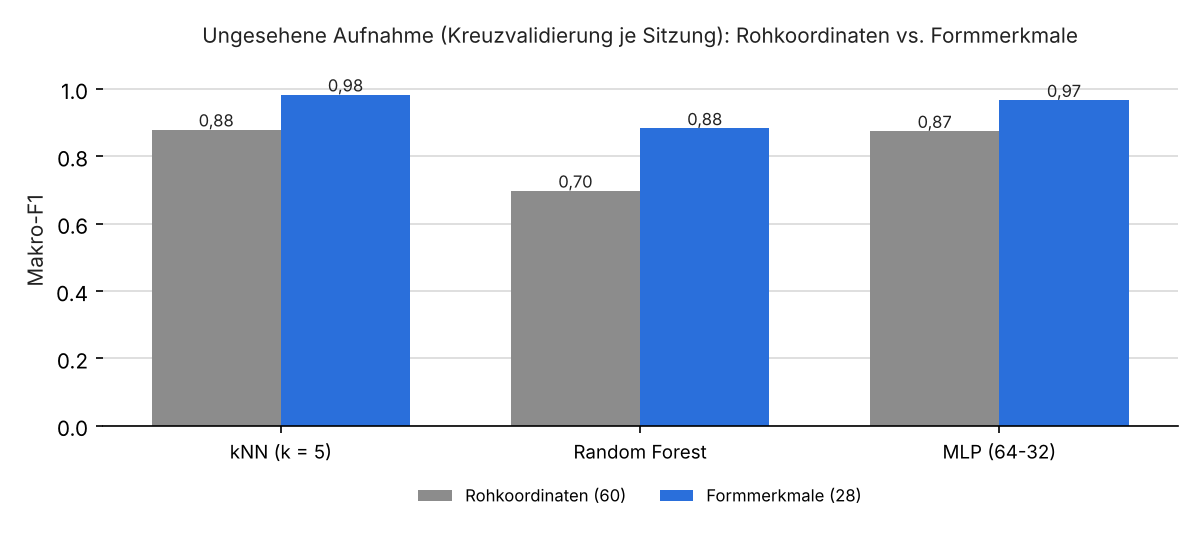
\includegraphics[width=0.9\textwidth]{merkmale_vergleich.png}
\caption{Makro-F1 auf jeweils ungesehener Trainingssitzung (Mittelwert über die drei Sitzungen):
Rohkoordinaten im Vergleich zu Formmerkmalen}
\label{fig:merkmale}
\end{figure}

\subsection{Verfahren und Validierung}

Verglichen wurden drei Verfahren aus scikit-learn\,\cite{sklearn}: k-nächste Nachbarn (kNN,
$k = 5$, mit Standardisierung), Random Forest (200 Bäume) und ein mehrschichtiges Perzeptron (MLP,
zwei verdeckte Schichten mit 64 und 32 Neuronen, mit Standardisierung).

Aufeinanderfolgende Kamerabilder sind nahezu gleich. Eine zufällige Aufteilung in Trainings- und
Testbilder würde daher fast identische Bilder in beiden Teilen enthalten und die Güte überschätzen.
Bewertet wurde deshalb mit einer \emph{Kreuzvalidierung je Sitzung} (Leave-one-session-out):
Training auf zwei Sitzungen, Bewertung auf der dritten, für jede Sitzung einmal. Zum Vergleich
wurde auch eine Kreuzvalidierung über 2-s-Abschnitte innerhalb der Aufnahmen berechnet.

\begin{table}[H]
\centering
\small
\begin{tabular}{lcccrr}
\toprule
 & \multicolumn{3}{c}{ausgelassene Sitzung} & & \\
\cmidrule(lr){2-4}
Verfahren & gedimmt & hell 100\,cm & hell 50\,cm & \textbf{Mittelwert} & 2-s-Abschnitte \\
\midrule
kNN ($k = 5$) & 0,997 & 0,978 & 0,972 & \textbf{0,982} & 0,994 \\
Random Forest & 0,996 & 0,845 & 0,806 & 0,882 & 0,997 \\
MLP (64-32) & 0,998 & 0,982 & 0,918 & 0,966 & 0,994 \\
\bottomrule
\end{tabular}
\caption{Makro-F1 der Kreuzvalidierung mit Formmerkmalen}
\label{tab:cv}
\end{table}

Die Abschnitte innerhalb der Aufnahmen bewerten alle Verfahren nahezu gleich gut, die Bewertung je
Sitzung zeigt dagegen deutliche Unterschiede. Der Random Forest passt sich am stärksten an die
Handhaltung einer einzelnen Sitzung an und verallgemeinert am schlechtesten. Ausgewählt wurde
anhand der Kreuzvalidierung je Sitzung (nicht anhand der Testsitzung) das kNN-Verfahren. Es
benötigt auf dem MacBook Air (M3) 0,3\,ms pro Bild, gegenüber etwa 13\,ms für die
MediaPipe-Verarbeitung insgesamt.

\subsection{Ergebnis auf der Testsitzung und Vergleich mit MediaPipe}

Die Testsitzung wurde von beiden Klassifikatoren mit denselben Bildern und denselben Schwellen
ausgewertet, zusätzlich auf Steuerungsebene durch den Zustandsautomaten wie im Betrieb.

\begin{table}[H]
\centering
\small
\begin{tabular}{lrr}
\toprule
 & Eigenes Modell (kNN) & MediaPipe \\
\midrule
Genauigkeit (Bildebene) & 100,0\,\% & 99,7\,\% \\
Makro-F1 & 1,000 & 0,997 \\
falsche Befehlsgeste (Anteil aller Bilder) & 0,0\,\% & 0,3\,\% \\
Befehlsgeste bei \enquote{keine Befehlsgeste} & 0,0\,\% & 2,2\,\% \\
richtiger Befehl ausgelöst (Steuerungsebene) & 7 / 7 & 7 / 7 \\
Befehle bei \enquote{keine Befehlsgeste} (Steuerungsebene) & 0 & 0 \\
\bottomrule
\end{tabular}
\caption{Testsitzung (728 Bilder): eigenes Modell und MediaPipe im Vergleich}
\label{tab:test}
\end{table}

Auf der Testsitzung ordnete das eigene Modell alle Bilder richtig zu. MediaPipe erkannte in zwei
Bildern ohne Befehlsgeste den Zeigefinger; auf Steuerungsebene führte dies wegen der Entprellung
zu keinem Befehl. Das MLP erreichte ebenfalls 100\,\%, der Random Forest nur 78,6\,\%.

\subsection{Bewertung und Grenzen}

\begin{itemize}
  \item Das eigene Modell ist auf diesen Daten mindestens gleichwertig zu MediaPipe. Die
        Testsitzung war mit 6\,s je Geste kurz und offenbar einfach (auch MediaPipe erreichte
        99,7\,\%). Aussagekräftiger ist daher der Mittelwert der Kreuzvalidierung je Sitzung von
        0,982.
  \item Das Modell wurde mit den Händen einer einzigen Person trainiert. MediaPipe ist auf vielen
        Personen trainiert und verallgemeinert daher voraussichtlich besser auf andere Bediener.
        Für einen allgemeinen Einsatz wären Aufnahmen weiterer Personen nötig.
  \item Bei der Kreuzvalidierung erkannte das MLP in einer Sitzung die offene Hand nur in etwa
        60\,\% der Bilder. Da der Stopp bereits nach zwei Bildern auslöst, wäre der Stopp dennoch
        ausgelöst worden; ein verpasster Stopp ist aber der kritischste Fehler. Die Stopp-Erkennung
        sollte daher nicht von einem einzelnen Modell abhängen (siehe Ausblick).
  \item Der Hauptnutzen liegt in der Erweiterbarkeit: Eine neue Geste erfordert nur eine weitere
        Aufnahme und ein erneutes Training, während der MediaPipe-Klassifikator auf seine sieben
        Gesten festgelegt ist.
\end{itemize}

Standard bleibt der MediaPipe-Klassifikator, da er umfangreich erprobt ist; das eigene Modell wird
über \texttt{erkennung.backend: eigen} aktiviert.

% ---------------------------------------------------------------- 7
\section{Inbetriebnahme und Bedienung}

\subsection{Einrichtung}

Voraussetzung ist Python 3.11 (unter macOS z.\,B. über Homebrew). Im Projektordner:
\begin{lstlisting}
python3.11 -m venv .venv
source .venv/bin/activate
pip install -r requirements.txt
\end{lstlisting}
Beim ersten Start wird das MediaPipe-Modell (ca. 8\,MB) automatisch nach \datei{models/}
heruntergeladen. Unter macOS muss dem Terminal der Kamerazugriff erlaubt werden.

\subsection{Programme}

\begin{lstlisting}
python gesture_demo.py                  # nur Gestenerkennung
python main.py                          # Gestensteuerung (Roboter laut config.yaml)
python scripts/test_steuerung.py        # automatischer Test der Steuerung
python scripts/test_bcap_verbindung.py  # Verbindungstest (real: IP aus config.yaml)
python scripts/test_bcap_verbindung.py --ip <IP>   # Verbindungstest Simulation
python main.py --roboter bcap --ip <IP>            # Gestensteuerung Simulation
python scripts/analyse_protokoll.py data/protokoll_X.csv --titel "Simulation" --ausgabe ergebnis_simulation.md

# eigener Klassifikator
python scripts/aufnahme_datensatz.py --sitzung train_hell_50cm   # je Sitzung
python scripts/aufnahme_datensatz.py --sitzung test_1 --dauer 6  # Testsitzung
python scripts/training_klassifikator.py   # Training, Bericht, Modell
python scripts/vergleich_merkmale.py       # Rohkoordinaten vs. Formmerkmale
python scripts/test_klassifikator.py       # Test der Merkmale
\end{lstlisting}

\subsection{Erprobung ohne Roboter: Simulation (VRC)}

Die Simulation benötigt Windows (hier Windows 11 in einer UTM-VM unter macOS) und das
COBOTTA-Softwarepaket von DENSO (Ordner \datei{Software}, Version 1.2.9). Die Lizenzschlüssel
stellt der Betreuer bereit; sie gehören nicht in das Repository. Bewährte Reihenfolge:
\begin{enumerate}
  \item \textbf{DENSO ROBOTICS License Manager} installieren (Ordner \datei{LicenseManager}) und
        den WINCAPS-III-Schlüssel eintragen.
  \item \textbf{VRC} installieren (Ordner \datei{VRC}); den VRC-Schlüssel im Lizenzdialog des
        Installers eingeben. (Im zuvor installierten License Manager wurde er als ungültig abgelehnt.)
  \item \textbf{WINCAPS III} aus dem vollständigen \datei{Software}-Ordner installieren, da das Setup
        weitere Installationsdateien im selben Verzeichnis erwartet. Dabei wird auch ORiN2 mit dem
        bCapListener installiert. Das ORiN2-Setup allein meldete \enquote{License is invalid}.
  \item \datei{TP.exe} (VRC) starten und \datei{Cobotta\_test.WPJ} öffnen.
  \item \datei{bCapListener.exe} (unter \datei{C:\textbackslash ORiN2\textbackslash CAO\textbackslash ProviderLib\textbackslash b-CAP})
        starten und die Firewall-Freigabe bestätigen; das Fenster während der Versuche geöffnet lassen.
  \item IP-Adresse der VM mit \texttt{ipconfig} ermitteln und vom Mac prüfen:
        \texttt{nc -vz <IP> 5007} muss \enquote{succeeded} melden.
  \item \texttt{python scripts/test\_bcap\_verbindung.py --ip <IP>}, danach
        \texttt{python main.py --roboter bcap --ip <IP>}.
\end{enumerate}

\subsection{Anbindung an einen realen COBOTTA}

\begin{enumerate}
  \item Rechner per Netzwerkkabel mit der Steuerung verbinden und eine feste IP-Adresse im Netz der
        Steuerung einstellen, z.\,B. 192.168.0.10, Subnetzmaske 255.255.255.0.
  \item An der Steuerung die Ausführungsberechtigung (Executable Token) für Ethernet freigeben.
  \item Arbeitsraumgrenzen in \datei{config.yaml} an den Aufbau anpassen.
  \item Falls ein elektrischer Greifer montiert ist: \texttt{greifer.vorhanden: true}.
  \item \datei{scripts/test\_bcap\_verbindung.py} ausführen. Das Skript verbindet sich, liest die
        Position, beobachtet sie 5\,s lang und fährt erst nach Bestätigung einen Schritt von 5\,mm in
        Z und zurück. Hand am Not-Halt behalten.
  \item In \datei{config.yaml} \texttt{roboter.backend: bcap} setzen und \datei{main.py} starten.
\end{enumerate}

\subsection{Bedienung}

Nach dem Start zeigt das Fenster das Kamerabild mit Zustand, aktiver Achse (farbig),
Schrittweite, erkannter Geste, Position und letzter Meldung. Ablauf: Faust halten (Freigabe),
mit dem Zeigefinger die Achse wählen, mit Daumen hoch/runter verfahren, mit dem I-love-you-Zeichen
zwischen 5\,mm und 1\,mm umschalten, mit der offenen Hand stoppen. Die Taste \texttt{q} beendet
das Programm; dabei wird der Roboter gestoppt und freigegeben.

% ---------------------------------------------------------------- 8
\section{Hinweise zur Weiterentwicklung}

\begin{itemize}
  \item \textbf{Andere Zuordnung der Gesten:} nur den Abschnitt \texttt{gesten} in \datei{config.yaml}
        ändern; es stehen die sieben MediaPipe-Gesten zur Verfügung.
  \item \textbf{Neue Geste (eigener Klassifikator):} Geste in \texttt{KLASSEN} in
        \datei{src/klassifikator.py} und \datei{scripts/aufnahme\_datensatz.py} ergänzen, alle
        Sitzungen neu aufnehmen, \datei{scripts/training\_klassifikator.py} ausführen und die Geste
        in \datei{config.yaml} einem Befehl zuordnen.
  \item \textbf{Neuer Befehl:} in \datei{src/controller.py} einen weiteren Zweig für den Befehl
        ergänzen, in \datei{src/safety.py} die zugehörige Prüfung und Ausführung, und den Test in
        \datei{scripts/test\_steuerung.py} erweitern.
  \item \textbf{Anderer Roboter} (z.\,B. igus ReBeL): eine neue Klasse von
        \texttt{RobotInterface} ableiten, die sechs Methoden implementieren und in
        \datei{src/robot/\_\_init\_\_.py} unter einem neuen Backend-Namen eintragen. Steuerung und
        Sicherheitsschicht bleiben unverändert.
  \item \textbf{Schwellen anpassen:} neue Aufnahmen mit \datei{scripts/aufnahme\_erkennung.py}
        erstellen, mit \datei{scripts/analyse\_erkennung.py} auswerten und die Werte in
        \datei{config.yaml} begründet anpassen.
\end{itemize}

% ---------------------------------------------------------------- 9
\section{Fazit und Ausblick}

Es wurde ein System entwickelt, mit dem ein DENSO COBOTTA berührungslos über sieben Handgesten
verfahren werden kann. Das Bedienkonzept überträgt den Tippbetrieb des Teach Pendants auf Gesten.
Das mehrstufige Sicherheitskonzept mit Freigabe, priorisiertem Stopp, Überwachung der Hand,
Entprellung und unabhängiger Sicherheitsschicht wurde durch 21 automatisierte Prüfungen bestätigt.
Die Gestenerkennung erreichte über 1416 Bilder und vier Aufnahmebedingungen eine Erkennungsrate
von 97,0\,\%. Verwechslungen zwischen Gesten traten nicht auf, und bei freier Handbewegung wurde
kein Bewegungsbefehl ausgelöst. Ein eigener, auf selbst aufgenommenen Daten trainierter
Klassifikator (kNN mit 28 Formmerkmalen) erreichte auf ungesehenen Sitzungen einen Makro-F1 von
0,982 und war auf der Testsitzung mindestens gleichwertig zum MediaPipe-Modell. Dabei zeigte sich,
dass eine Bewertung innerhalb derselben Aufnahmen die Güte überschätzt und dass Merkmale, die die
Form der Hand beschreiben, deutlich besser verallgemeinern als die rohen Koordinaten.
In der Simulation mit der virtuellen DENSO-Steuerung lief die vollständige Kette über b-CAP:
236 Schritte wurden exakt ausgeführt, der Stopp löste nach 35\,ms aus, und alle Schritte über die
Arbeitsraumgrenzen hinaus wurden abgelehnt.

Grenzen des Systems:
\begin{itemize}
  \item Es wird nur die Position des Werkzeugs verändert, nicht seine Orientierung.
  \item Die Reaktionszeit wird durch die Bildrate der Kamera begrenzt (15 Bilder/s bei wenig Licht).
  \item Die Bewegung wird synchron ausgeführt; während eines Schritts wird kein neues Bild
        ausgewertet. Ein Stopp wirkt daher erst nach dem laufenden Schritt (in der Simulation bis
        0,58\,s bei 5\,mm und 0,26\,s bei 1\,mm).
  \item Die Software-Sicherheitsfunktionen ersetzen keine zertifizierte Sicherheitstechnik.
\end{itemize}

Mögliche Erweiterungen:
\begin{itemize}
  \item zusätzliche Gesten mit dem eigenen Klassifikator, z.\,B. zur Steuerung der Orientierung,
        sowie Aufnahmen weiterer Personen,
  \item redundante Stopp-Erkennung: Stopp, sobald MediaPipe \emph{oder} das eigene Modell die
        offene Hand erkennt (zwei unabhängige Verfahren für die wichtigste Funktion),
  \item asynchrone Bewegung mit sofortigem Abbruch während eines Schritts,
  \item eine Kamera mit höherer Bildrate für kürzere Reaktionszeiten,
  \item kontinuierliches Verfahren, solange eine Geste gehalten wird.
\end{itemize}

% ---------------------------------------------------------------- Quellen
\begin{thebibliography}{9}
\bibitem{mediapipe} Google: \emph{MediaPipe Gesture Recognizer}. Online-Dokumentation,
  \url{https://developers.google.com/edge/mediapipe/solutions/vision/gesture_recognizer}
\bibitem{orinbcap} DENSO WAVE: \emph{orin\_bcap – b-CAP-Client-Bibliotheken (C, C\#, Java, Python)}.
  MIT-Lizenz, \url{https://github.com/DENSORobot/orin_bcap}
\bibitem{opencv} OpenCV: \emph{Open Source Computer Vision Library}. \url{https://opencv.org}
\bibitem{sklearn} Pedregosa, F. u.\,a.: \emph{Scikit-learn: Machine Learning in Python}. Journal of
  Machine Learning Research 12 (2011), S.~2825--2830. \url{https://scikit-learn.org}
\end{thebibliography}

% ---------------------------------------------------------------- Anhang
\appendix
\section{Konfigurationsdatei}
\label{anh:config}
\lstinputlisting{../../config.yaml}

\end{document}
